\documentclass{beamer}

% This file is a solution template for:

% - Talk at a conference/colloquium.
% - Talk length is about 20min.
% - Style is ornate.



% Copyright 2004 by Till Tantau <tantau@users.sourceforge.net>.
%
% In principle, this file can be redistributed and/or modified under
% the terms of the GNU Public License, version 2.
%
% However, this file is supposed to be a template to be modified
% for your own needs. For this reason, if you use this file as a
% template and not specifically distribute it as part of a another
% package/program, I grant the extra permission to freely copy and
% modify this file as you see fit and even to delete this copyright
% notice. 


\mode<presentation>
{
  % \usetheme{Warsaw}
  % or ...

  \setbeamercovered{transparent}
  % or whatever (possibly just delete it)
}


\usepackage[english]{babel}
% or whatever

\usepackage[utf8]{inputenc}
% or whatever

\usepackage{url}


%\usepackage{times}
%\usepackage[T1]{fontenc}
% Or whatever. Note that the encoding and the font should match. If T1
% does not look nice, try deleting the line with the fontenc.


\title % (optional, use only with long paper titles)
{FOSS4G-CEE 2013}

% \subtitle {Include Only If Paper Has a Subtitle}

%\author[Jachym Cepicky] % (optional, use only with lots of authors)
%{Jáchym~Čepický\inst{1}}
% - Give the names in the same order as the appear in the paper.
% - Use the \inst{?} command only if the authors have different
%   affiliation.

%\institute[HSRS] % (optional, but mostly needed)
%{
%  \inst{1}%
%  Help Service - Remote Sensing\\
%  \url{http://bnhelp.cz}\\
%  \url{jachym@bnhelp.cz}
%}
% - Use the \inst command only if there are several affiliations.
% - Keep it simple, no one is interested in your street address.

%\date[] % (optional, should be abbreviation of conference name)
%{FOSS4G-CEE, 2012}
% - Either use conference name or its abbreviation.
% - Not really informative to the audience, more for people (including
%   yourself) who are reading the slides online

%\subject{FOSS4G-CEE Closing words}
% This is only inserted into the PDF information catalog. Can be left
% out. 


% If you have a file called "university-logo-filename.xxx", where xxx
% is a graphic format that can be processed by latex or pdflatex,
% resp., then you can add a logo as follows:

\pgfdeclareimage[height=0.75cm]{logo}{imgs/logo}
%\logo{\pgfuseimage{logo}}


% Delete this, if you do not want the table of contents to pop up at
% the beginning of each subsection:
%\AtBeginSubsection[]
%{
%  \begin{frame}<beamer>{Outline}
%    \tableofcontents[currentsection,currentsubsection]
%  \end{frame}
%}


% If you wish to uncover everything in a step-wise fashion, uncomment
% the following command: 

%\beamerdefaultoverlayspecification{<+->}


\begin{document}

\begin{frame}
  \titlepage
  \only<1>{
    
\includegraphics[height=75px]{imgs/logo}
}
    \only<2>{
    
\includegraphics[height=75px]{imgs/logo-foss4g-cee-2013.png}
}
\end{frame}

%\begin{frame}{Outline}
%  \tableofcontents
%  % You might wish to add the option [pausesections]
%\end{frame}


% Structuring a talk is a difficult task and the following structure
% may not be suitable. Here are some rules that apply for this
% solution: 

% - Exactly two or three sections (other than the summary).
% - At *most* three subsections per section.
% - Talk about 30s to 2min per frame. So there should be between about
%   15 and 30 frames, all told.

% - A conference audience is likely to know very little of what you
%   are going to talk about. So *simplify*!
% - In a 20min talk, getting the main ideas across is hard
%   enough. Leave out details, even if it means being less precise than
%   you think necessary.
% - If you omit details that are vital to the proof/implementation,
%   just say so once. Everybody will be happy with that.

%\section{Introduction}

%\begin{frame}{Presentations}{}
%  \begin{center}
%    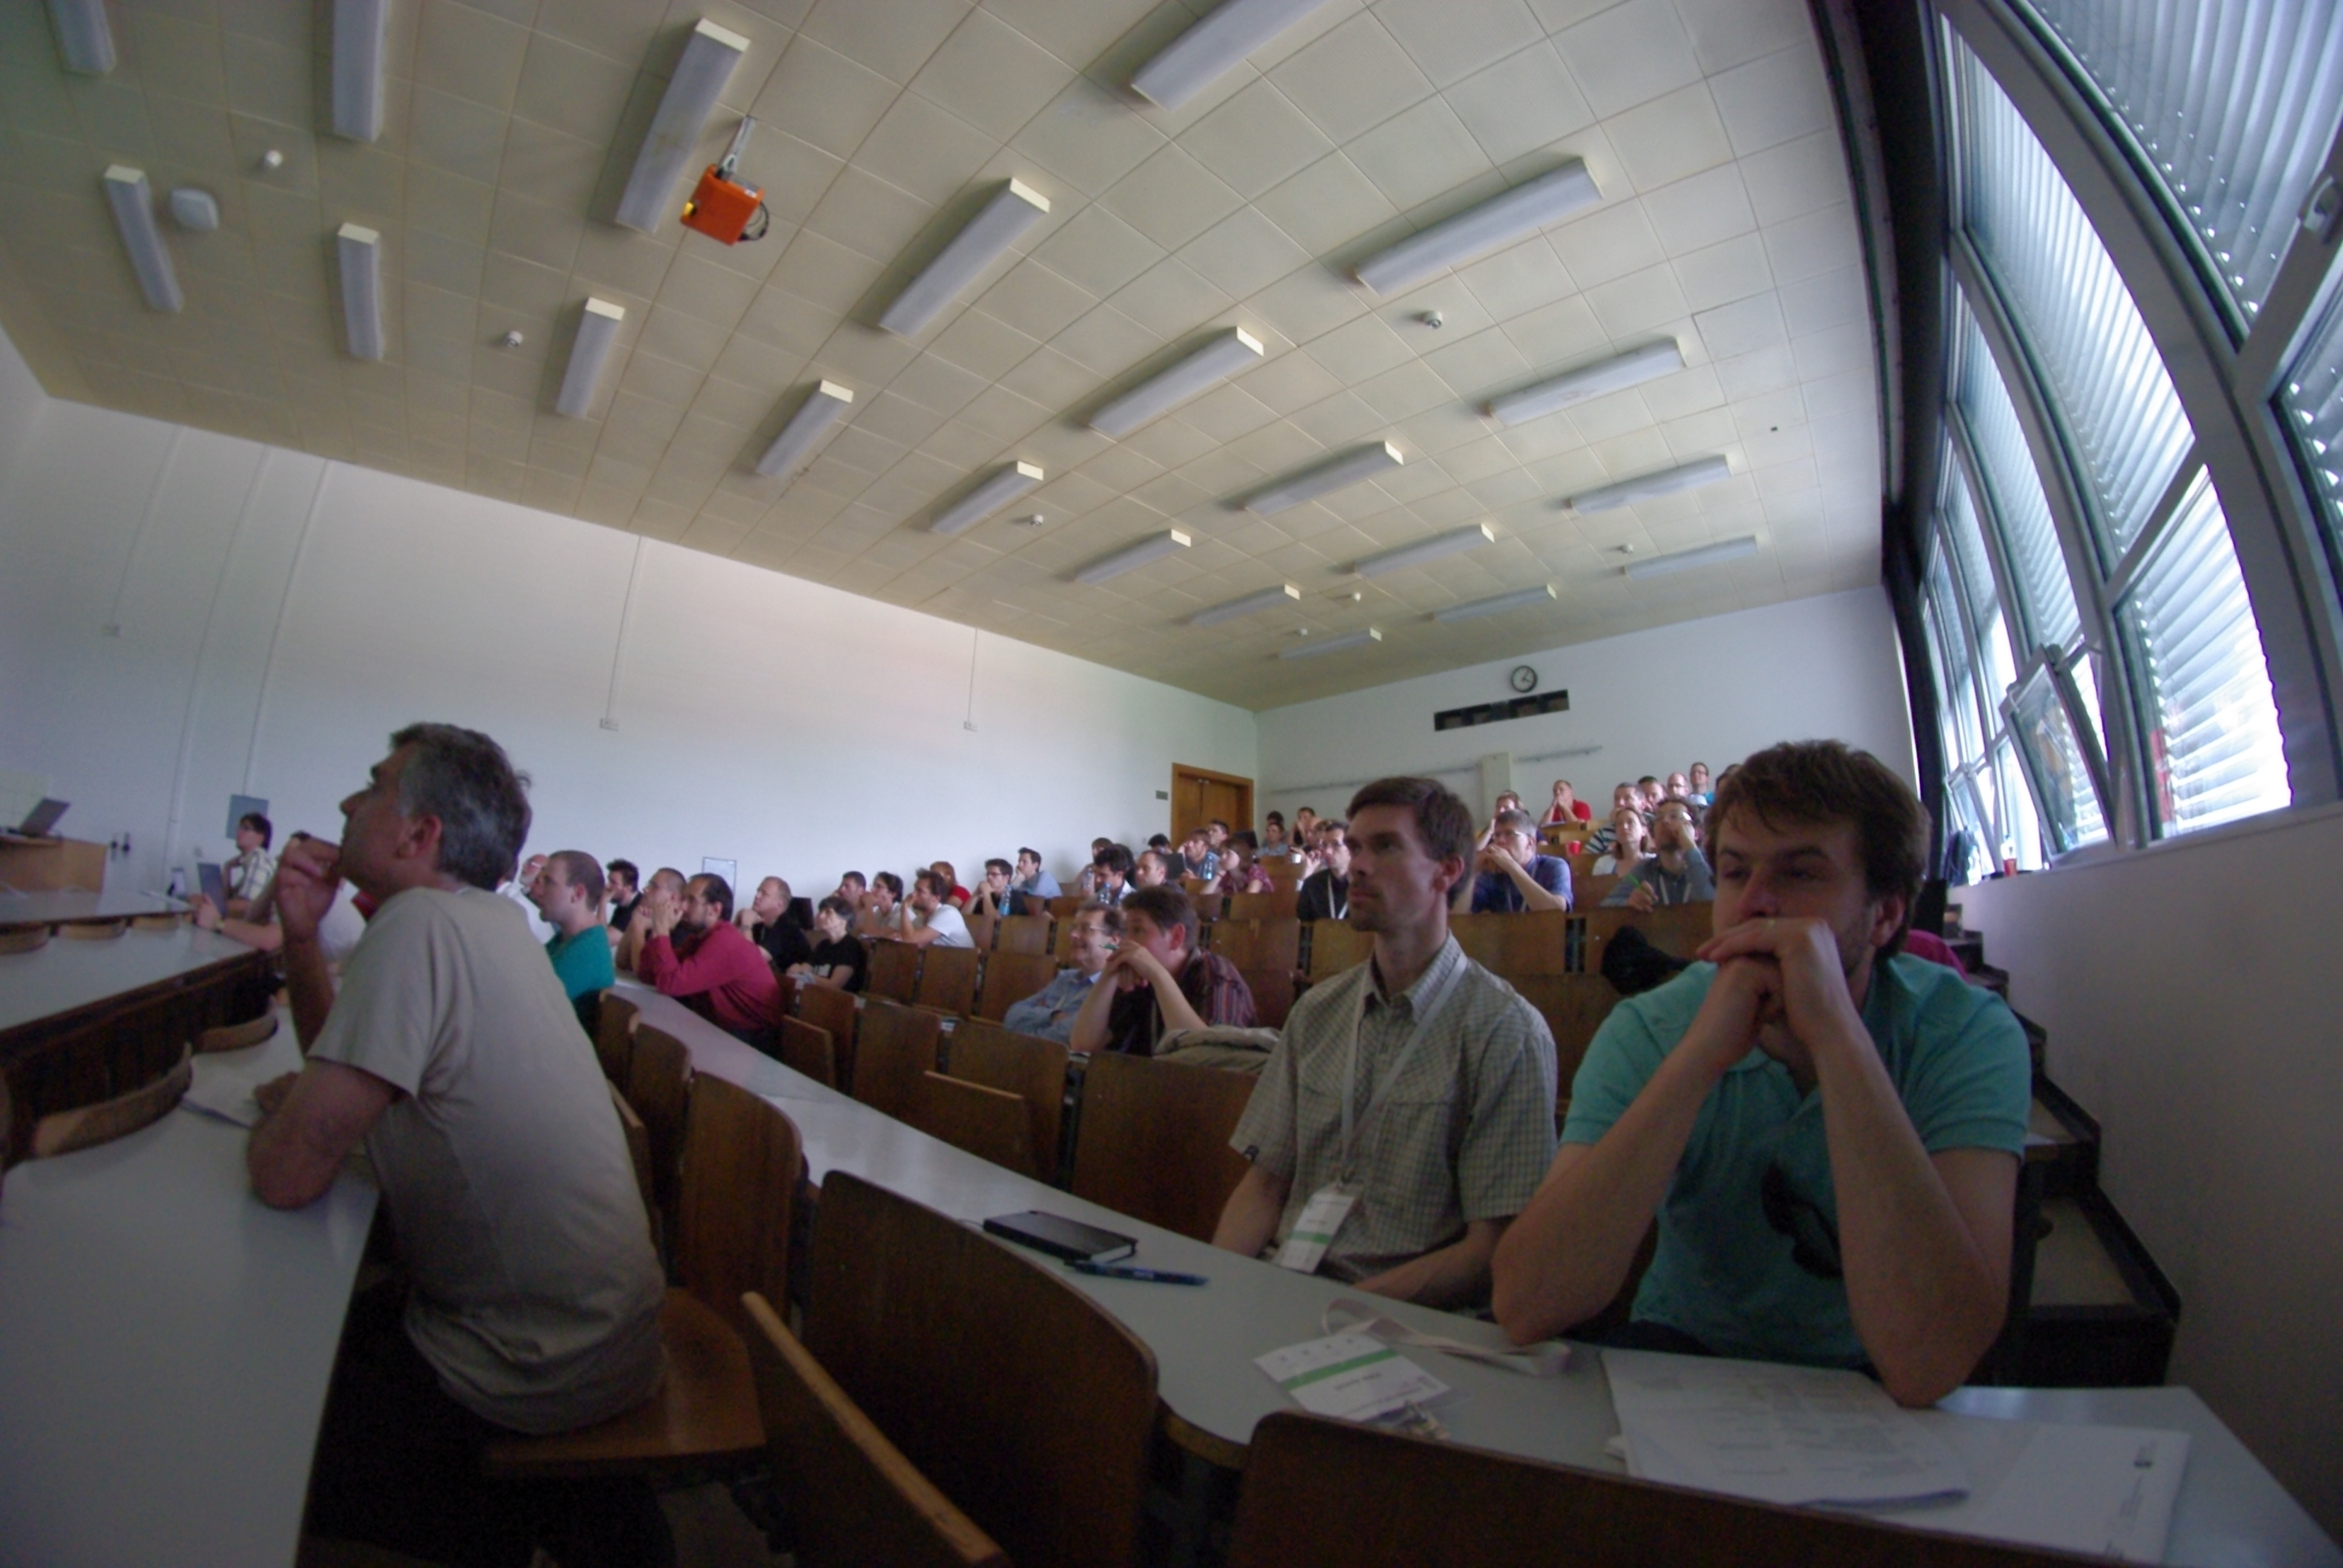
\includegraphics[height=200px]{imgs/listening.jpg}
%  \end{center}
%\end{frame}
%
%%\begin{frame}{Fun}{}
%%  \begin{center}
%%    \includegraphics[height=300px]{imgs/fun.jpg}
%%
%%  \end{center}
%%\end{frame}
%
%\begin{frame}{Social}{}
%  \begin{center}
%    \includegraphics[height=200px]{imgs/social.jpg}
%
%  \end{center}
%\end{frame}
%
%\begin{frame}{Working}{}
%  \begin{center}
%    \includegraphics[height=200px]{imgs/working.jpg}
%
%  \end{center}
%\end{frame}
%
%\begin{frame}{Friends}{}
%  \begin{center}
%    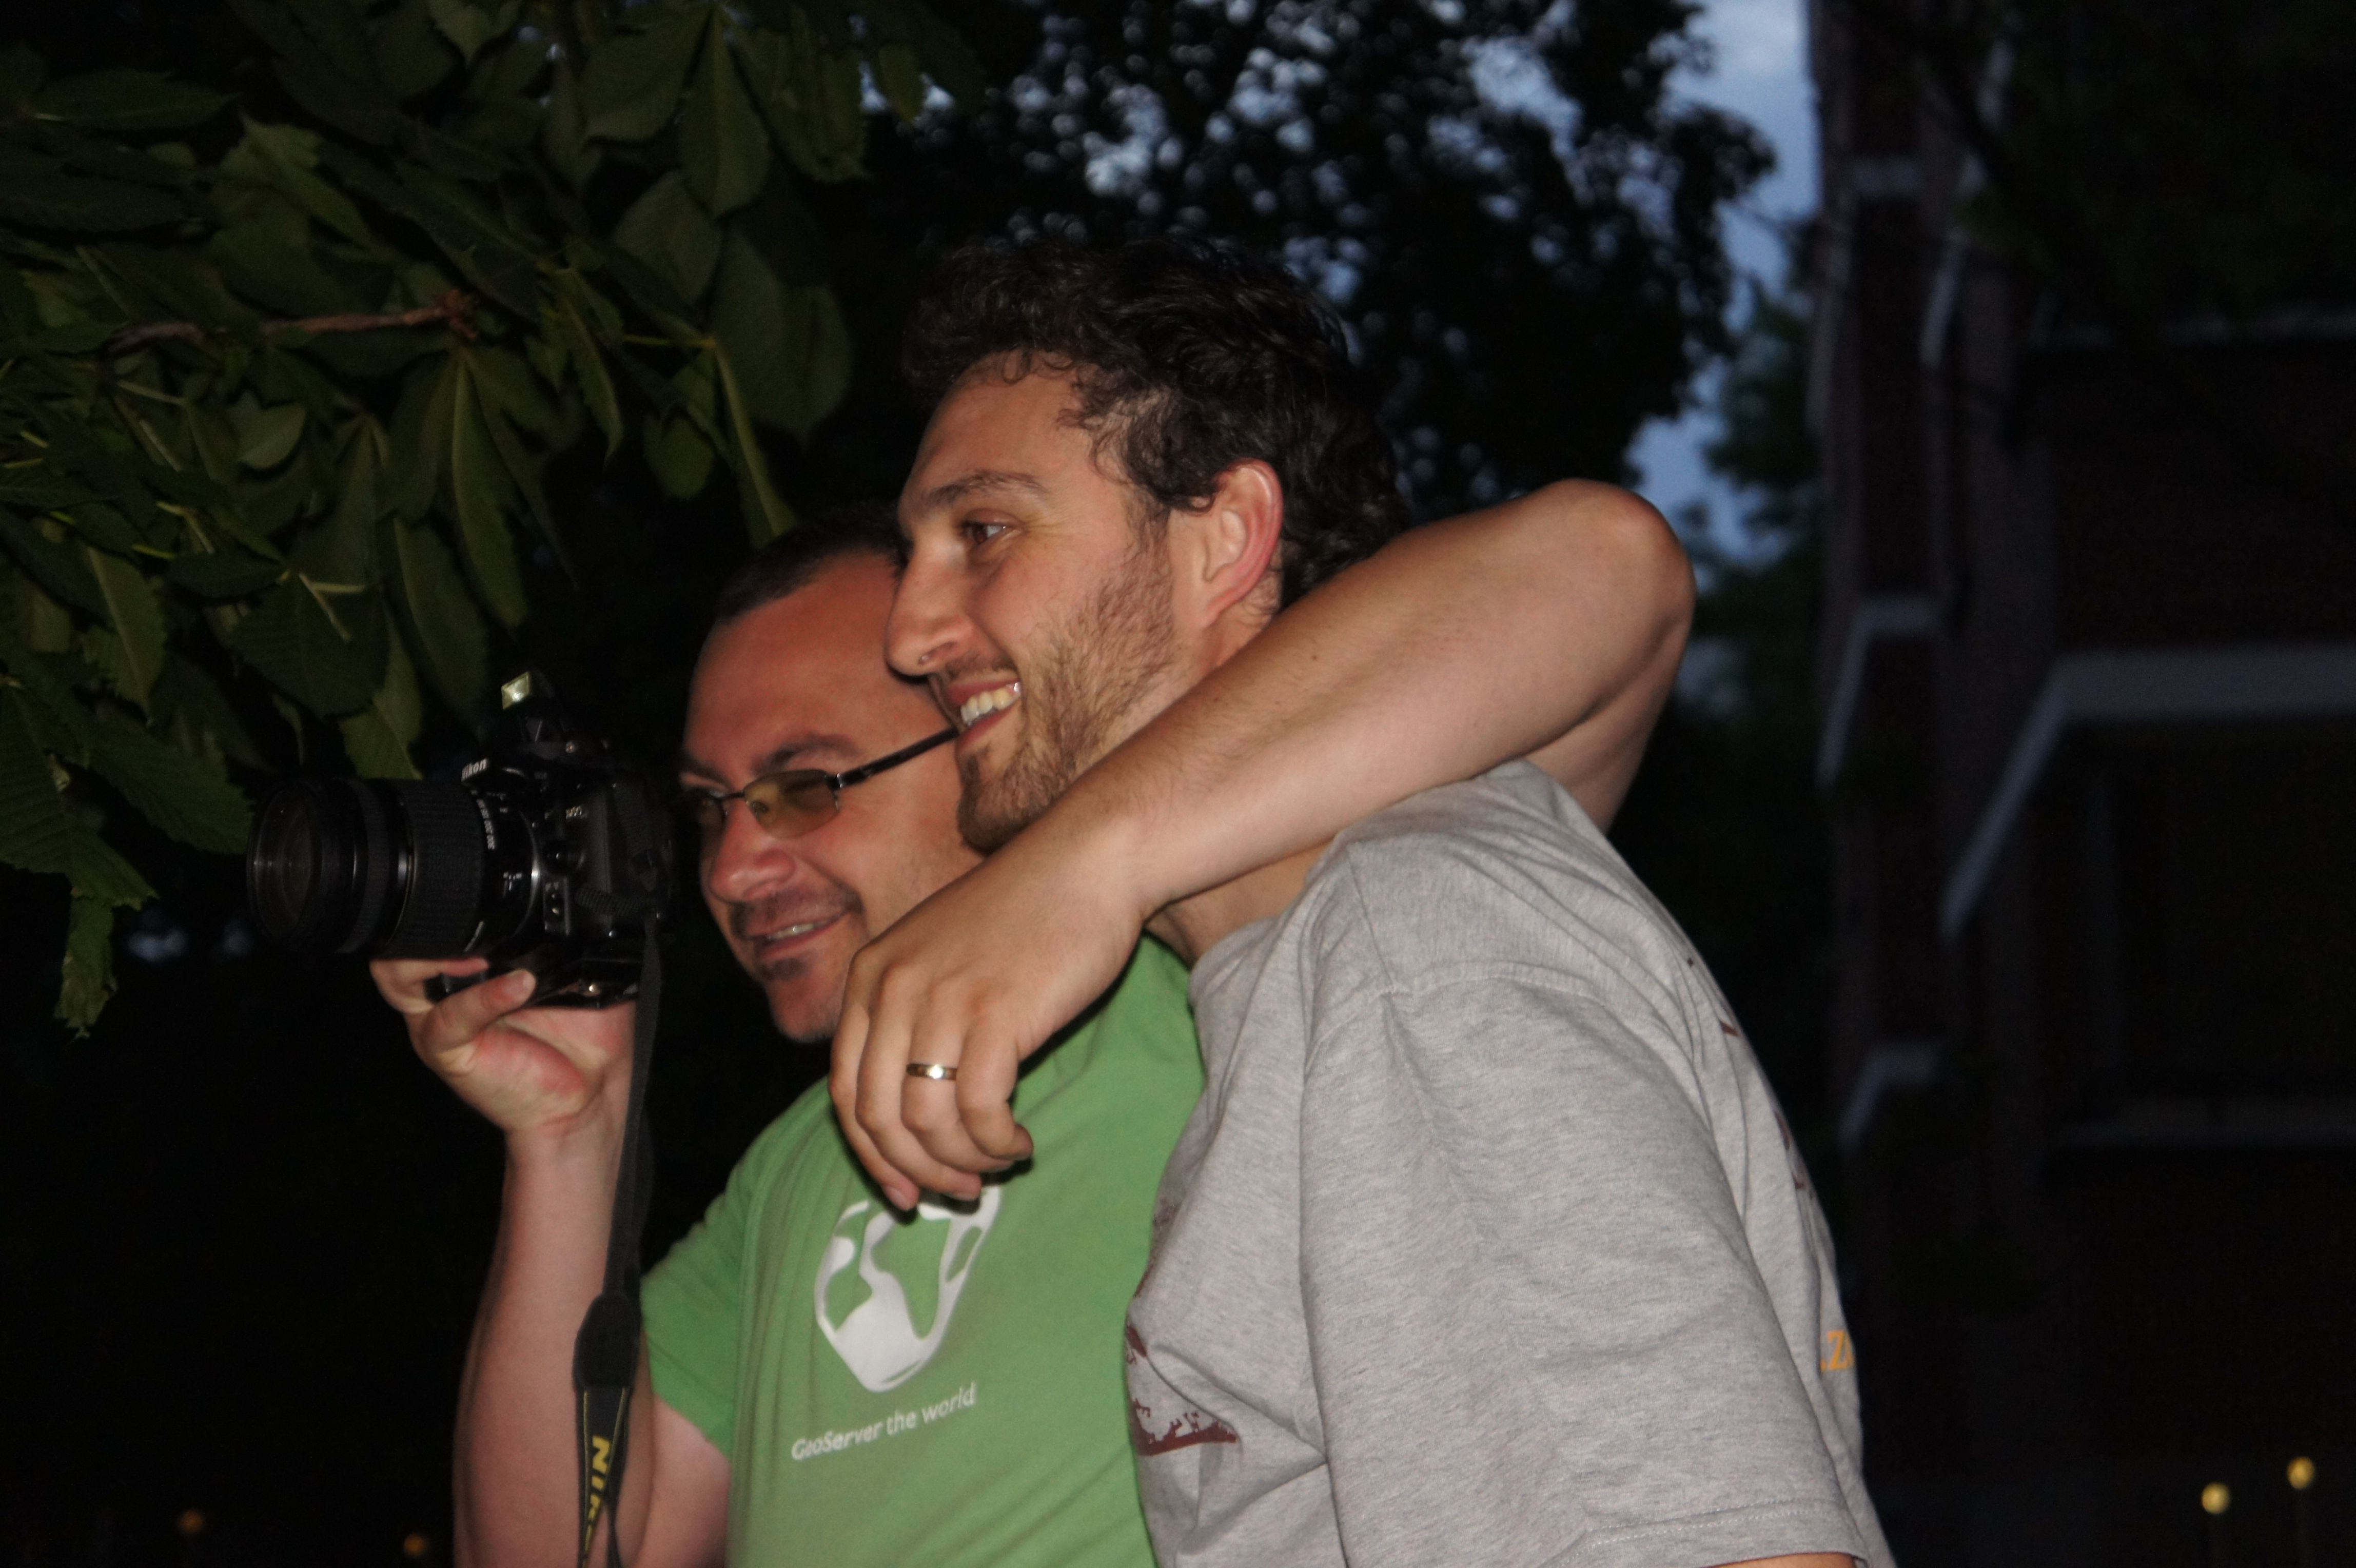
\includegraphics[height=200px]{imgs/friends.jpg}
%
%  \end{center}
%\end{frame}
%
%\begin{frame}{Homeworks}{}
%  \begin{itemize}
%	\item Presentations 
%	\item Photos
%  \end{itemize}
%foss4g-cee@foss4g-cee.org
%\end{frame}
%
%
%\begin{frame}{End}{}
%  \begin{center}
%    \includegraphics[height=200px]{imgs/odchod.jpg}
%
%  \end{center}
%\end{frame}

\begin{frame}{Outlook}{}
  \begin{center}
    \includegraphics[height=200px]{imgs/outlook.jpg}

  \end{center}
\end{frame}

\begin{frame}{Outlook}{}
  \begin{center}
    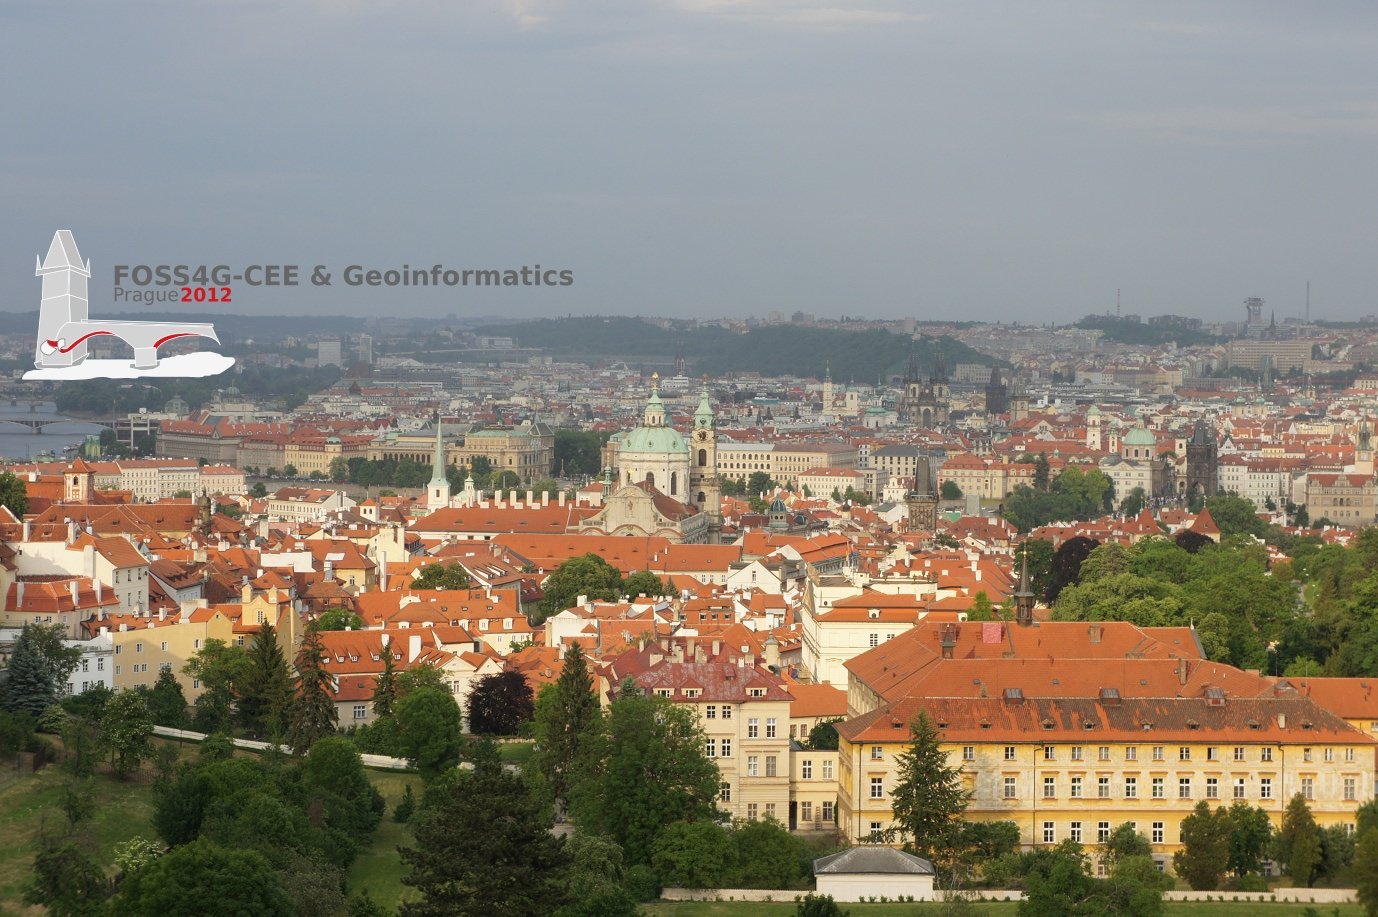
\includegraphics[height=200px]{imgs/outlook1.jpg}

  \end{center}
\end{frame}

\begin{frame}{Outlook}{}
  \begin{center}
    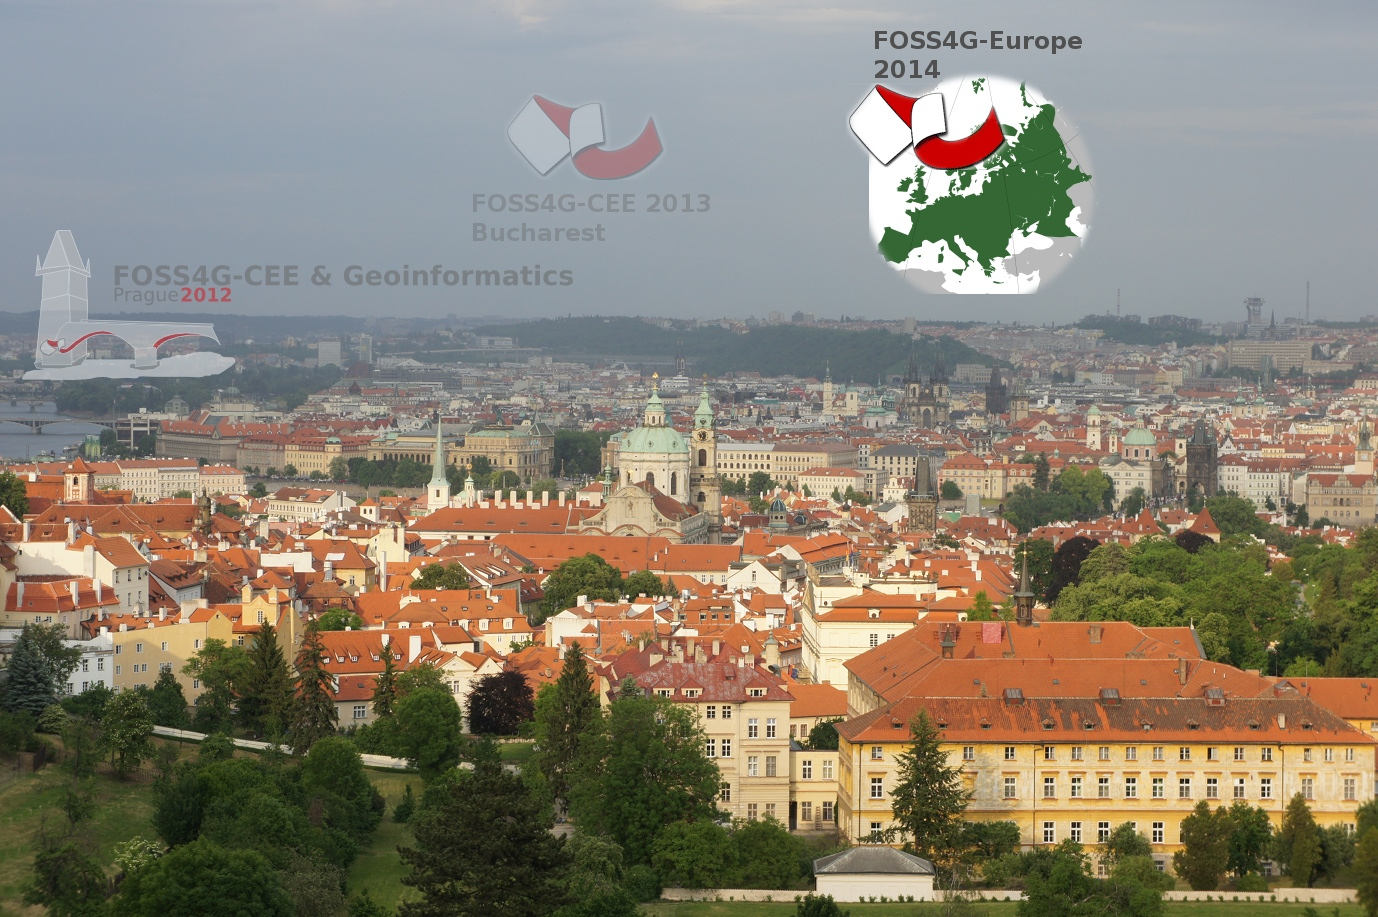
\includegraphics[height=200px]{imgs/outlook3.jpg}

  \end{center}
\end{frame}
\begin{frame}{FOSS4G-Europe?}{} \begin{center}
    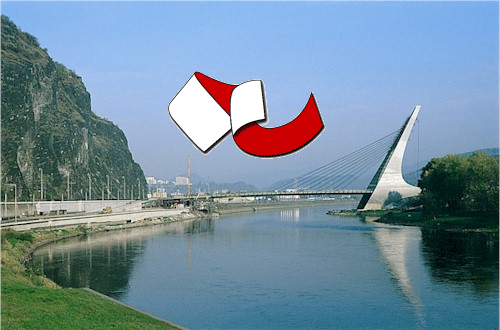
\includegraphics[height=200px]{imgs/most.png}

  \end{center}
\end{frame}

%
%
%\begin{frame}{Media}{}
%  \begin{center}
%      
\includegraphics[height=200px]{imgs/media.png}
%  \end{center}
%\end{frame}
%
%\begin{frame}{Org. Team}{}
%  \begin{center}
%      
\includegraphics[width=100px]{imgs/ccss.png} \vfill
%      
\includegraphics[width=100px]{imgs/hsrs.png} \vfill
%      
\includegraphics[height=60px]{imgs/cenia.png}
%  \end{center}
%\end{frame}
%
%\begin{frame}{CTU}{}
%  \begin{center}
%      
%      
\includegraphics[height=100px]{imgs/cvut.png}
%
%      \url{http://cvut.cz}
%
%  \end{center}
%\end{frame}
%
%\begin{frame}{OSGeo}{}
%  \begin{center}
%      
\includegraphics[height=100px]{imgs/osgeo.png}
%
%      \url{http://osgeo.org}
%  \end{center}
%\end{frame}
%
%
%\begin{frame}{}{}
%  \begin{center}
%      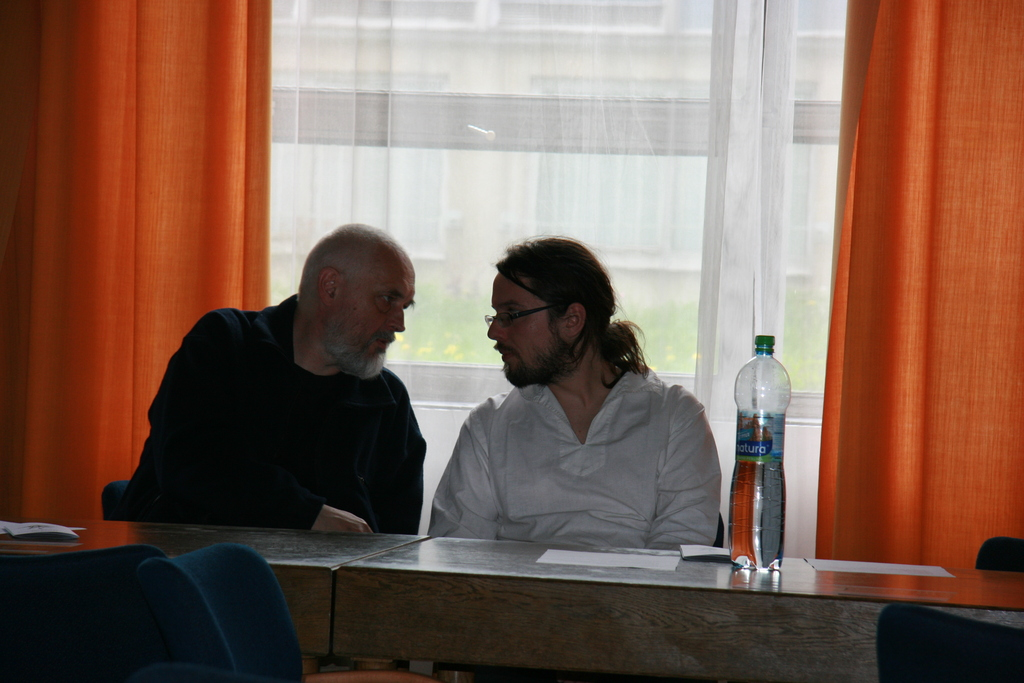
\includegraphics[height=100px]{imgs/cepek.png}
%	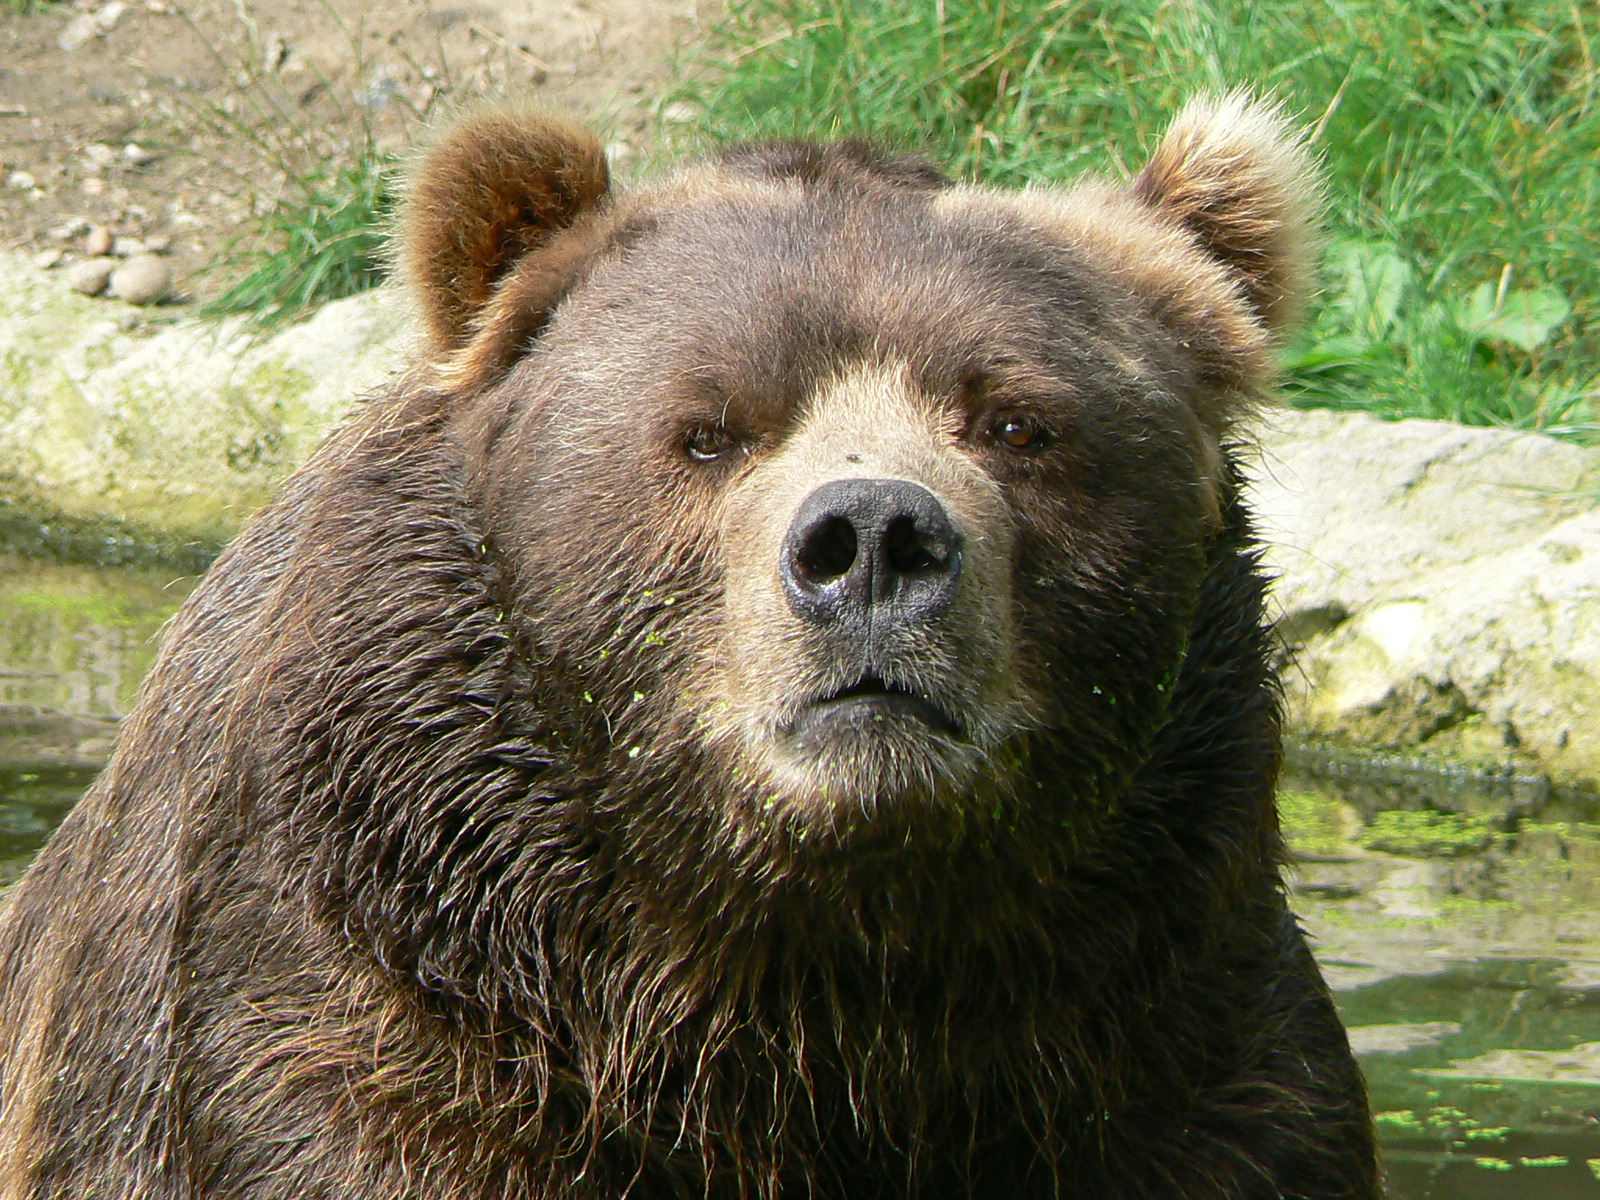
\includegraphics[height=100px]{imgs/krivanek.png}
%
%	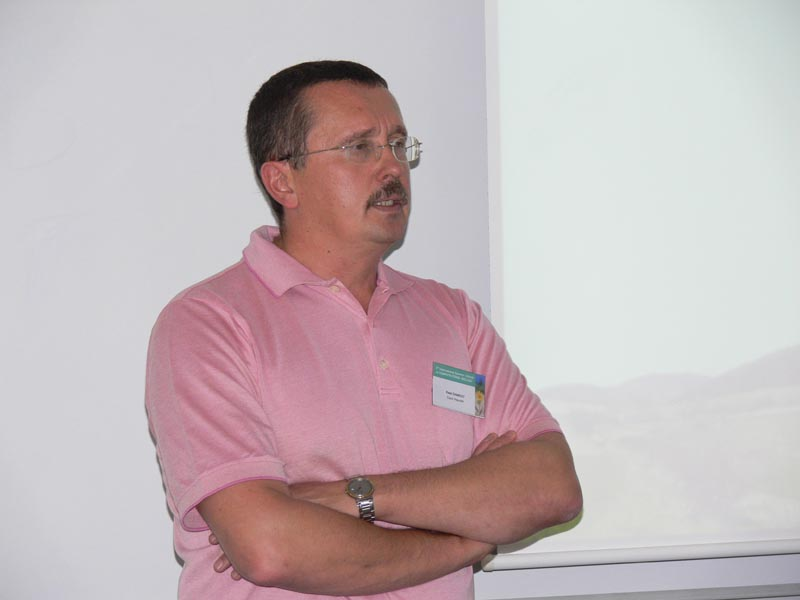
\includegraphics[height=100px]{imgs/charvat.png}
%  \end{center}
%\end{frame}

\begin{frame}{}{}
  \begin{center}
      Thank you!
  \end{center}
\end{frame}

\begin{frame}{Enjoy!}{}
  \begin{center}
      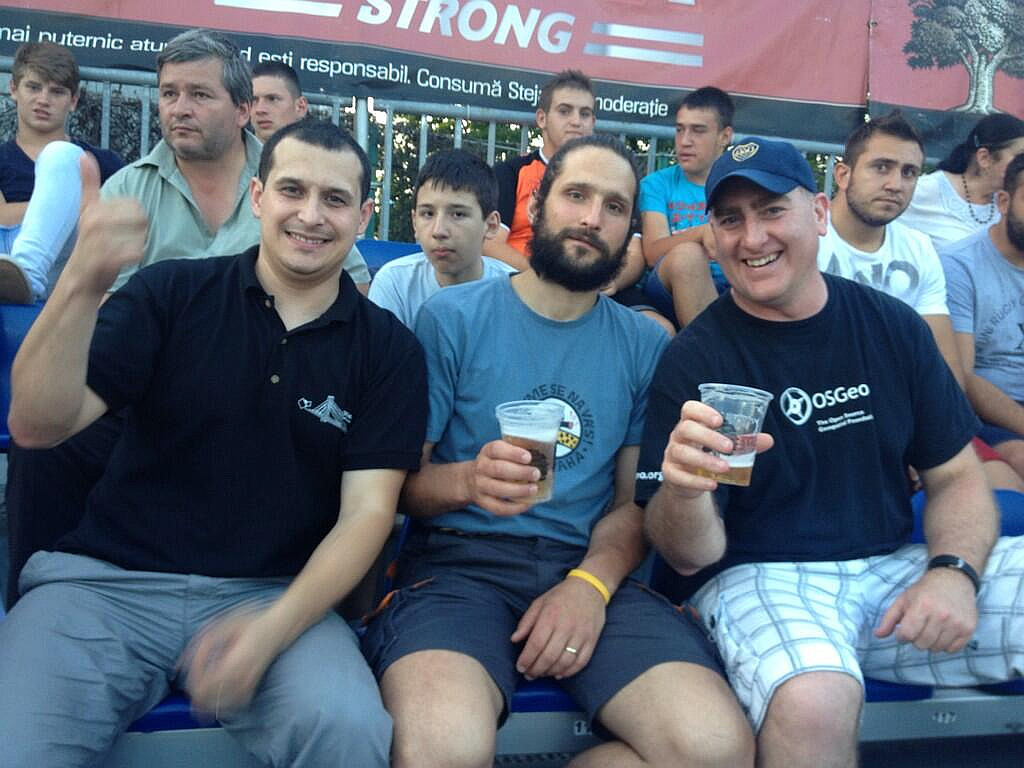
\includegraphics[height=200px]{imgs/enjoy.jpg}\\
      \#work \#social
  \end{center}
\end{frame}

\end{document}


